\chapter[Elicitação de Requisitos]{Elicitação de Requisitos}

  Existem muitas técnicas de elicitação, 
  que consistem em adquirir conceitos e informações importantes afim de formar um conhecimento 
  comum entre cliente e desenvolvedores. A seguir apresentaremos as técnicas escolhidas pelo grupo.
    
  \section{Definição das Técnicas de Elicitação}
  
    Existem três questões-chave para definição das técnicas de elicitação de requisitos para um projeto
    de acordo com Leffingwell e Widrig (\citeyear{leffingwell99}). São elas:
    
    \begin{itemize}
     \item A síndrome “Sim, mas...” emerge da natureza humana e da falta do software ser algo palpável.
     \item Procurar por requisitos é como procurar por “ruínas não-descobertas”, quanto mais você encontra, mais você sabe que permanece sem ser descoberto.
     \item A síndrome do “Usuário e o Desenvolvedor” que reflete as diferenças profundas entre os dois,dificultando a comunicação.
    \end{itemize}
    
    Atentando para esses 3 problemas, as técnicas escolhidas para o projeto, foram explicadas de acordo com  Leffingwell e Widrig (\citeyear{leffingwell99}), e são elas: entrevista, \textit{workshop} e \textit{brainstorming}.
    
    \subsection{Entrevista}
      
      Pontos-Chave
    
      \begin{itemize}
       \item Entrevista é uma técnica simples e direta. 
       \item Questões sem contexto podem ajudar atingir resultados mais puros e não direcionados.
       \item Convergências em algumas necessidades comuns vão iniciar um “repositório de requisitos” para ser usado durante o projeto. 
       \item Um questionário não é um substituto para uma entrevista.
      \end{itemize}
    
      A entrevista é uma técnica muito poderosa e pode ser utilizada virtualmente em qualquer contexto, 
      mas ela força a aproximação direta com a síndrome “Usuário e o Desenvolvedor” 
      fazendo com que sua aplicação não seja uma tarefa trivial.

      Durante a entrevista é normal que o entrevistador faça perguntas guiadas pela solução que ele já imaginou para a situação, 
      afinal ele é pago para ter essa noção, 
      mas essa prática pode tirar o foco do real problema sendo exposto pelo cliente 
      pelo simples motivo do entrevistador já ter resolvido muitos problemas parecidos 
      anteriormente e estar imaginando como resolver esse sem nem ainda saber qual é. 
      A partir disso como fazemos para não atrapalhar as respostas do usuário com perguntas? 
      Fazendo perguntas da natureza do problema do usuário sem contexto para uma possível solução. 
      Para conseguir isso,  Leffingwell e Widrig (apud Gause, (\citeyear{gause89})) introduziu o conceito das 
      “Questões sem contexto”, como por exemplo:
      
      \begin{itemize}
       \item Quem é o usuário?
       \item Quem é o consumidor?
       \item As necessidades deles são diferentes?
       \item Onde mais uma solução para esse problema pode ser encontrada?
      \end{itemize}
      
      Essas questões forçam o entrevistador a ouvir antes de tentar inventar ou descrever uma potencial solução. 
      Ouvir nos dá um melhor entendimento dos problemas do consumidor e qualquer problema por trás desse problema. 
      Esses problemas afetam a motivação do usuário e precisam ser identificados antes de podermos entregar uma solução eficaz.
    
      Essa técnica é utilizada em vendas na técnica de vender soluções, 
      quando o vendedor aplica maior esforço na primeira abordagem ao cliente para efetivamente identificar quais são os problemas deste, 
      e a partir disso vender aquilo que mais se identifica como a solução para aquele problema.
    
      Mas é claro que o cliente depende do trabalho do entrevistador para guiar a entrevista 
      para o campo onde o usuário identifica os problemas, caso contrário o usuário ensinaria 
      tudo o que sabe para o entrevistador, que absorveria pouco para resolução do problema.
      
    \subsection{\textit{Workshop} de requisitos}
    
      Pontos-chave:
      \begin{itemize}
       \item Reúne os \textit{stakeholders} mais importantes por um pequeno período de tempo, mas intensamente focado.
       \item O uso de um facilitador experiente na gerência dos requisitos pode ajudar a assegurar o sucesso do \textit{workshop}.
       \item O \textit{brainstorm} é a parte mais importante do \textit{workshop}.
      \end{itemize}
      
      O \textit{workshop} de requisitos é designado para encorajar o consenso dos requisitos da aplicação 
      e para adquirir um rápido acordo no curso das ações, 
      tudo em um tempo reduzido. Com essa técnica, os \textit{stakeholders} mais importantes para o projeto são 
      reunidos por um curto e intenso período, geralmente não mais do que 1 ou 2 dias. 
      A atividade é facilitada por um membro do time, ou melhor, 
      um facilitador de fora da equipe experiente e foca na criação ou revisão das features de alto nível 
      para serem entregues pela nova aplicação.
      
      Alguns pontos são observados quando se utiliza do \textit{workshop} da forma correta:
      \begin{itemize}
       \item Ajuda na construção de um time efetivo, comprometido com um objetivo em comum: o sucesso desse projeto.
       \item Todos os \textit{stakeholders} tem sua voz e vez, nenhum é deixado de fora.
       \item Produz um acordo entre os \textit{stakeholders} e a equipe de desenvolvimento de o que a aplicação fará.
       \item Pode expor e resolver problemas políticos que estão interferindo com o sucesso do projeto.
       \item Produz uma definição preliminar do sistema no nível de funcionalidades.
      \end{itemize}
      
      Agora serão listados alguns passos-modelo para planejar e executar com sucesso o \textit{workshop} de requisitos.
      \subsubsection{Preparação}
	
	Na fase de preparação será necessário vender a ideia do \textit{workshop} encorajando os \textit{stakeholders} 
	a participarem de fato da atividade.
	
	Ainda na preparação é necessário decidir quais são os \textit{stakeholders} corretos para participarem do \textit{workshop}.
	
	É importante arquitetar e observar os pontos de logística que se aplicam ao evento, 
	cuidar de tudo desde o lugar do encontro, transporte, convite oficial até a iluminação da sala do \textit{workshop}. 
	Trabalhar com profissionalismo e foco ajudam nessa fase.
	
	É necessário disponibilizar documentos que ajudem no aquecimento do \textit{workshop}, 
	podem ser disponibilizados pontos, como numa agenda, para ajudar no decorrer da atividade, 
	como por exemplo rascunhos dos documentos de requisitos, lista de funcionalidades sugeridas, 
	copias das entrevistas com usuários de prospecção, cartas de consumidores, novas diretivas de gerenciamento, 
	entre outros. É importante não enterrar todos em documentos, mas entregar somente o que for necessário. 
	Outra parte do aquecimento é convidar a todos esquecer por um momento todos os limites formais do projeto 
	e simplesmente coletar ideias de novas funcionalidades e estar preparado para abstrair em um nível mais alto. 
	O líder do \textit{workshop} pode incitar as ideias e criatividade dos participantes mostrando artigos sobre requisitos 
	criativamente. 
	Nessa atmosfera, soluções criativas serão os resultados.
      
      \subsubsection{Papel do facilitador}
	
	O facilitador deve ser uma pessoa que já tem algum treinamento do processo e demostrou um pensamento 
	de construção de senso ou habilidade de construção de times, 
	além de ser respeitado por todos os membros e conseguir lidar com uma reunião desafiadora. 
	Pode ser um membro do time, enquanto facilitador, este não deverá contribuir para as ideias e problemas na reunião. 
	Ou então o \textit{workshop} estará em grande perigo de perder a objetividade que é necessária para chegar aos fatos reais
	e não estará em um ambiente de confiança onde o consenso emerge.
	
	As responsabilidades do facilitador são:
	\begin{itemize}
	 \item Estabelecer um tom profissional e objetivo à reunião.
	 \item Estabelecer um tom profissional e objetivo à reunião.
	 \item Começar e terminar a reunião na hora certa.
         \item Estabelecer e reforçar as regras da reunião.
         \item Introduzir os objetivos e a agenda da reunião.
         \item Gerenciar a reunião e manter o time no caminho certo.
	 \item Facilitar o processo de decisão e consenso, mas evitar participar do conteúdo.
	 \item Gerenciar qualquer problema de logística para assegurar que o foco permaneça na agenda.
	 \item Se assegurar que todos os \textit{stakeholders} participem e tenham suais ideias sejam ouvidas.
	 \item Controlar comportamento disruptivo ou improdutivo.
	\end{itemize}
	
      \subsubsection{Definindo a Agenda}
	
	A agenda da reunião se baseará nas necessidades do projeto e o conteúdo que precisa ser desenvolvido no \textit{workshop}. 
	Nenhuma agenda cobre todos os problemas. 
	Entretanto, \textit{workshop}s de requisitos mais estruturados podem seguir um formato, como no exemplo abaixo:
	\begin{figure}[!htbp]
	  \centering
	  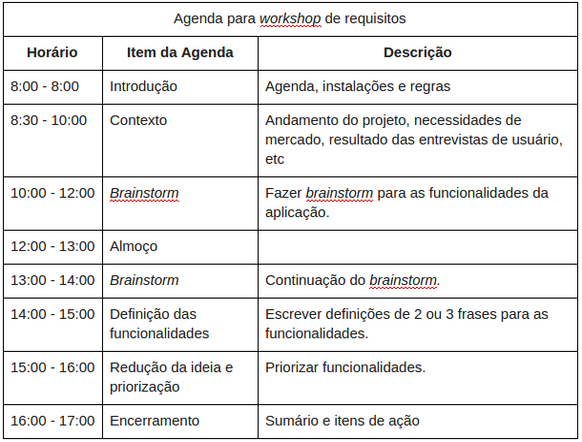
\includegraphics[scale=0.5]{editaveis/figuras/agenda_example}
	  \caption[Exemplo de agenda para \textit{workshop} de requisitos]
	    {Exemplo de agenda para \textit{workshop} de requisitos.\footnotemark}
	  \label{agenda_example}
	\end{figure}
	\footnotetext{Fonte: \cite{leffingwell99} }
	
      \subsubsection{Executando o \textit{workshop}}
      
	A reunião pode se tornar muito inquieta e muitos problemas podem surgir a partir disso. 
	Algumas técnicas podem ajudar nesse ponto afim de tornar a reunião um pouco mais descontraída 
	em um ambiente um pouco menos pesado para a equipe. 
	Uma boa técnica são os tickets. Eles são pedaços de papel com alguns atributos interessantes, 
	Leffingwell e Widrig(\citeyear{leffingwell99}) sugerem estes abaixo:
	
	\begin{figure}[!htbp]
	  \centering
	  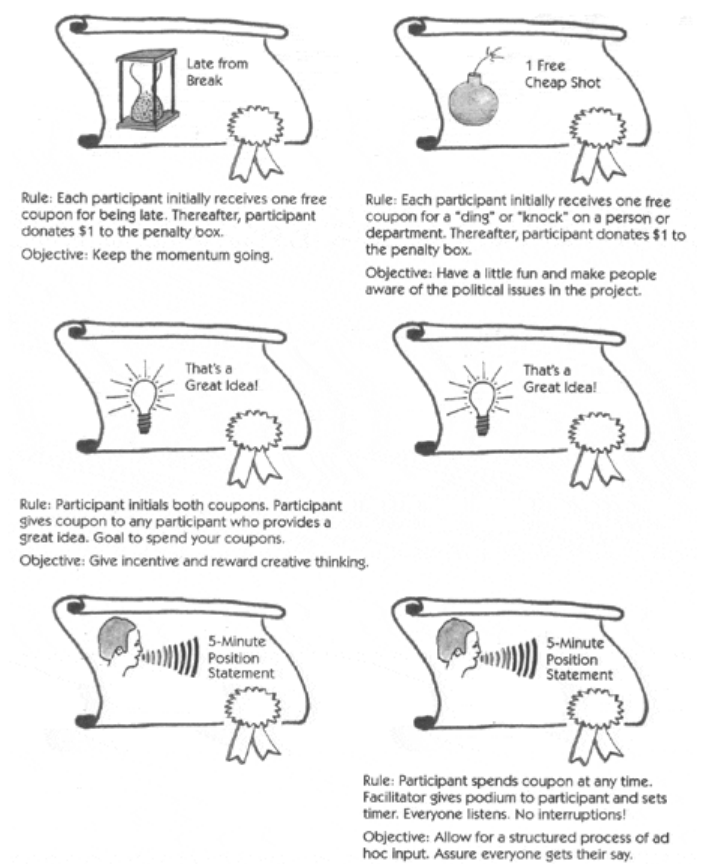
\includegraphics[scale=0.3]{editaveis/figuras/tickets}
	  \caption[Exemplo de tickets a serem usados no \textit{workshop}]
	    {Exemplo de tickets a serem usados no \textit{workshop}.\footnotemark}
	  \label{tickets}
	\end{figure}
	\footnotetext{Fonte: \cite{leffingwell99} }
	
	Vale lembrar que o facilitador deve introduzir essas regras e explicar a 
	dinâmica de uso dos tickets durante a reunião e alcançar um acordo de uso dos mesmos.
	
      \subsubsection{\textit{Brainstorm}}
	
	Essa prática envolve geração de ideias e redução de ideias, que gera muitas soluções criativas, 
	que resultam da combinação de múltiplas ideias e aparentemente sem relação entre elas. 
	Técnicas de votação podem ser utilizadas para priorizar funcionalidades.
      
      \subsubsection{Produção e seguimento}
      
	Após o \textit{workshop} o facilitador distribui os resultados da reunião e os grava. 
	Então, o trabalho do facilitador está terminado e a responsabilidade do sucesso está de novo nas mãos do time de desenvolvimento. 
	Leffingwell e Widrig(\citeyear{leffingwell99}) fornece um exemplo do quadro feito pelo facilitador:
	
	\begin{figure}[!htbp]
	  \centering
	  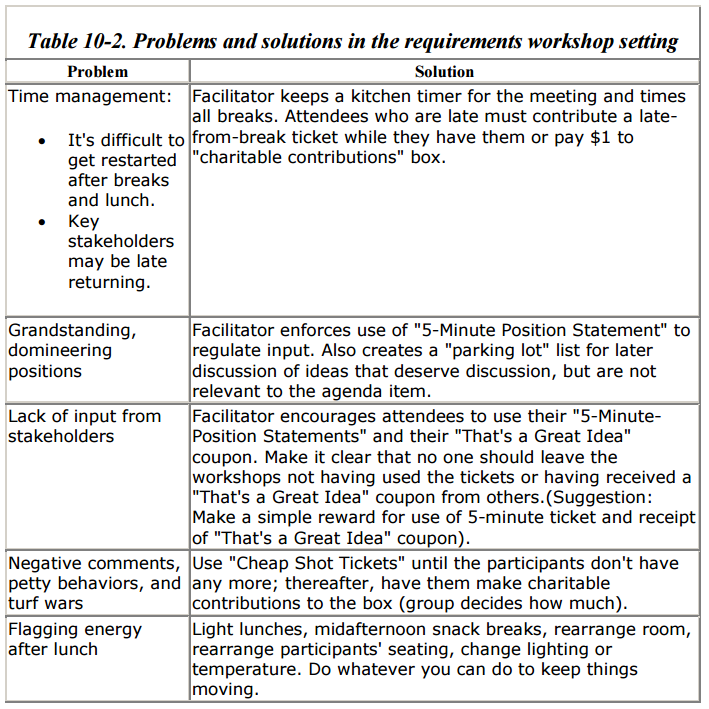
\includegraphics[scale=0.3]{editaveis/figuras/problems_solutions}
	  \caption[Exemplo do quadro redigido pelo facilitador]
	    {Exemplo do quadro redigido pelo facilitador.\footnotemark}
	  \label{problems_solutions}
	\end{figure}
	\footnotetext{Fonte: \cite{leffingwell99} }
	
	Depois disso o líder do projeto tem a responsabilidade de acompanhar qualquer ação que foram gravados 
	na reunião para organizar a informação para distribuição aos interessados. 
	Sempre, o resultado da reunião será uma lista simples de ideias ou funcionalidades de produtos 
	sugeridos que podem ser transformados imediatamente em ações para o time de desenvolvimento.
      
      


    


 
    